\pdfoptionpdfminorversion=5
\documentclass[spanish,professionalfonts]{beamer}
\usepackage{lmodern}
\usepackage[utf8]{inputenc}
\usepackage[english]{babel}
\usepackage{amsmath}
\usepackage{amssymb}
\usepackage{color}
\usepackage{xmpmulti}
\usefonttheme[onlymath]{serif}
\usepackage{tabularx}
\usepackage{listings}
%%Regular colours! 
\definecolor{MyBlack}{RGB}{0,0,0}
\definecolor{MyRed}{RGB}{255,0,0}
\definecolor{MyBlue}{RGB}{0,0,255}
\definecolor{MyGreen}{RGB}{0,200,0}
\definecolor{MyBrown}{RGB}{130,70,0}
\definecolor{MyPurple}{RGB}{120,0,160}
\definecolor{MyDarkPurple}{RGB}{100,0,140}
\definecolor{MyLightPurple}{RGB}{190,0,220}
\definecolor{MyYellow}{RGB}{170,170,0}
\definecolor{MyOrange}{RGB}{200,100,0}
\definecolor{MyCyan}{RGB}{0,200,200}
\definecolor{MyGray}{RGB}{220,220,220}
\definecolor{MyWhite}{RGB}{255,255,255}
\definecolor{MyInvisible}{RGB}{255,255,255}
\definecolor{MyPink}{RGB}{255,0,100}


%%Inverted colours!
%\definecolor{MyBlack}{RGB}{250,250,250}
%\definecolor{MyRed}{RGB}{0,230,230}
%\definecolor{MyBlue}{RGB}{170,110,0}
%\definecolor{MyGreen}{RGB}{255,0,255}
%\definecolor{MyBrown}{RGB}{120,175,255}
%\definecolor{MyPurple}{RGB}{70,190,40}
%\definecolor{MyLightPurple}{RGB}{70,190,40}
%\definecolor{MyDarkPurple}{RGB}{140,255,125}
%\definecolor{MyYellow}{RGB}{0,0,240}
%\definecolor{MyOrange}{RGB}{60,175,255}
%\definecolor{MyGray}{RGB}{200,200,200}
%\definecolor{MyWhite}{RGB}{5,5,5}
%\definecolor{MyInvisible}{RGB}{255,255,255}
%\definecolor{MyPink}{RGB}{0,255,150}

\usetheme{Boadilla}

\usepackage{calligra}
%\setbeamercovered{dynamic}
%\useoutertheme{shadow}
\useinnertheme{rectangles}
\usecolortheme[MyPurple]{structure}
\setbeamercolor{structure}{bg=MyGray, fg=MyDarkPurple}
\setbeamercolor{frametitle}{bg=MyInvisible, fg=MyBlue}
\setbeamercolor{title}{bg=MyPurple, fg=MyWhite}
%\setbeamercolor{normal text}{bg=MyBlack,fg=MyWhite}
%\setbeamercolor{alerted text}{fg=orange}
%\setbeamercolor{background canvas}{bg=black}
%\setbeamercolor{titlelike}{fg=MyBrown}
%\setbeamercolor{section in sidebar}{fg=MyRed}
%\setbeamercolor{section in sidebar shaded}{fg= grey}
%\setbeamercolor{subsection in sidebar}{fg=blue}
%\setbeamercolor{subsection in sidebar shaded}{fg= grey}
%\setbeamercolor{sidebar}{bg=red}

\setbeamertemplate{navigation symbols}{}%remove navigation symbols

\def\tcr#1{\textcolor{MyRed}{#1}}
\def\tcb#1{\textcolor{MyBlue}{#1}}
\def\tcbck#1{\textcolor{MyBlack}{#1}}
\def\tcg#1{\textcolor{MyGreen}{#1}}
\def\tcgr#1{\textcolor{MyGray}{#1}}
\def\tcbr#1{\textcolor{MyBrown}{#1}}
\def\tcp#1{\textcolor{MyPurple}{#1}}
\def\tcy#1{\textcolor{MyYellow}{#1}}
\def\tco#1{\textcolor{MyOrange}{#1}}
\def\tcc#1{\textcolor{MyCyan}{#1}}
\def\tcw#1{\textcolor{MyWhite}{#1}}
\def\tci#1{\textcolor{MyInvisible}{#1}}
\def\tcpk#1{\textcolor{MyPink}{#1}}

\def\NS{{\mathrm{NoSplit}}}
\def\ff{{\mathrm{MaxChoiceCols}}}
\def\Av{{\mathrm{Avoid}}}
\def\I{{\mathcal{I}}}
\newcommand{\ncols}[1]{\| #1 \|}
\def\qed{ \hskip 20pt{$\blacksquare$}\hfil}
\def\forb{{\mathrm{forb}}}
\def\cA{{\mathcal{A}}}
\def\cB{{\mathcal{B}}}
\def\cC{{\mathcal{C}}}
\def\cD{{\mathcal{D}}}
\def\cE{{\mathcal{E}}}
\def\cF{{\mathcal{F}}}
\def\cG{{\mathcal{G}}}
\def\cH{{\mathcal{H}}}
\def\cI{{\mathcal{I}}}
\def\cJ{{\mathcal{J}}}
\def\cK{{\mathcal{K}}}
\def\cL{{\mathcal{L}}}
\def\cM{{\mathcal{M}}}
\def\cN{{\mathcal{N}}}
\def\cO{{\mathcal{O}}}
\def\cP{{\mathcal{P}}}
\def\cQ{{\mathcal{Q}}}
\def\cR{{\mathcal{R}}}
\def\cS{{\mathcal{S}}}
\def\cT{{\mathcal{T}}}
\def\cU{{\mathcal{U}}}
\def\cV{{\mathcal{V}}}
\def\cW{{\mathcal{W}}}
\def\cX{{\mathcal{X}}}
\def\cY{{\mathcal{Y}}}
\def\cZ{{\mathcal{Z}}}

\def\I{{\mathcal{I}}}

\def\CC{{\mathbb{C}}}
\def\HH{{\mathbb{H}}}
\def\RR{{\mathbb{R}}}
\def\NN{{\mathbb{N}}}
\def\ZZ{{\mathbb{Z}}}
\def\QQ{{\mathbb{Q}}}
\def\Var{{\mathrm{Var}}}
\def\cov{{\mathrm{cov}}}
\def\corr{{\mathrm{corr}}}

\newtheorem{nota}{Note}
\newtheorem{problema}{Problem}
\newtheorem{teorema}{Theorem}
\newtheorem{proposicion}{Proposition}
\newtheorem{ejercicio}{Exercise}
\newtheorem{definicion}{Definition}
\newtheorem{propiedad}{Property}
\newtheorem{principio}{Principle}
\newtheorem{observacion}{Observation}
\newtheorem{pregunta}{Question}
\newtheorem{lema}{Lemma}
\newtheorem{ejemplo}{Example}
\newtheorem{formula}{Formula}

\title{Discreture}
\author{Miguel Raggi \\ \texttt{mraggi@gmail.com}}
\institute{Escuela Nacional de Estudios Superiores \\ UNAM}
\subtitle{A \textbf{C++} library to generate \tcg{simple} combinatorial objects}
% \date{2 de marzo}
\usepackage{tikz}
\setbeamertemplate{button}{\tikz
  \node[
  inner xsep=10pt,
  draw=structure!80,
  fill=structure!50,
  rounded corners=4pt]  {\Large\insertbuttontext};}

\begin{document}

\AtBeginSection[]
{
\begin{frame}
\frametitle{Index}
\tableofcontents[currentsection]
\end{frame} 
}

\begin{frame}
\begin{center}
\large{\tcg{\textbf{Software Tools for Mathematics}}}
\end{center}
\titlepage
\end{frame}

\begin{frame}
\frametitle{Index}
\tableofcontents
\end{frame} 

\section{Motivation}

\begin{frame}\frametitle{What is discreture?}
  \begin{definicion}
    \tcp{Discreture} is an open source C++ library to produce combinatorial objects like \textbf{combinations}, \textbf{set-partitions}, \textbf{motzkin paths}, etc.
  \end{definicion}

  \begin{center}
   \url{https://github.com/mraggi/discreture}
  \end{center}  \pause

  \begin{itemize}
    \item You can use it for (pretty much) any purpose (Apache license). \pause
    \item It has a focus on \tcg{ease of use}, \tcp{compatibility with the STL}, \tcg{speed} and \tcg{correctness} \pause (not necessarily in that order).\pause
    \item \tcr{Contributor:} Manuel Alejandro Romo de Vivar.
  \end{itemize}

\end{frame}

\defverbatim[colored]\codeone{\begin{center}
\begin{lstlisting}[language=C++,basicstyle=\ttfamily,keywordstyle=\color{blue},otherkeywords={*,vector,std},commentstyle=\color{MyYellow},tabsize=4]
    int n = 20;
    for (int i = 0; i < n; ++i)
    {
      for (int j = i+1; j < n; ++j)
      {
        // Do stuff
      }
    }
\end{lstlisting}\end{center}
}

\begin{frame}\frametitle{Motivation}
  \begin{itemize}
    \item Suppose you wish to do something with \tcp{every pair of objects} in a set\pause
    \item Easy:    
    \codeone
  \end{itemize}
\end{frame}

\begin{frame}\frametitle{Motivation}
  \begin{itemize}
    \item Now, what if you want all triples? 
    \item Easy: just add another for loop.\pause
    \item Quadruples? Quintuples?
  \end{itemize}
\end{frame}

\defverbatim[colored]\codetwo{\begin{center}
\begin{lstlisting}[language=C++,basicstyle=\ttfamily,keywordstyle=\color{blue},otherkeywords={*,vector,std},commentstyle=\color{MyYellow},tabsize=1]
  int n = 20;
  for (int i = 0; i < n; ++i)
  {
    for (int j = i+1; j < n; ++j)
    {
      for (int k = j+1; j < n; ++k)
      {
        for (int l = k+1; l < n; ++l)
        {
          for (int m = l+1; m < n; ++m)
          {
             // Do stuff
          }  
        }
      }
    }
  }
\end{lstlisting}\end{center}
}
\begin{frame}\frametitle{Quintuples?}
  \codetwo
\end{frame}

\defverbatim[colored]\codethree{\begin{center}
\begin{lstlisting}[language=C++,basicstyle=\ttfamily,keywordstyle=\color{blue},otherkeywords={*,vector,std},commentstyle=\color{MyYellow},tabsize=2]
  for (auto& x : combinations(20,5))
  {
    // Do stuff with x[0], x[1], ...
  }
\end{lstlisting}\end{center}
}

\begin{frame}\frametitle{A better solution}
  This is what it looks like in discreture:
  \codethree
\end{frame}

\defverbatim[colored]\codefour{\begin{center}
\begin{lstlisting}[language=C++,basicstyle=\ttfamily,keywordstyle=\color{blue},otherkeywords={*,std},commentstyle=\color{MyYellow},tabsize=2]
  std::vector<MyObject> A;
  
  //... fill A somehow
  
  for (auto x : compound_combinations(A,5))
  {
    // x[i] has type MyObject&
  }
\end{lstlisting}\end{center}
}

\begin{frame}\frametitle{Not just indices}
  Or maybe:
  \codefour
\end{frame}

\subsection{Supported combinatorial objects}
\begin{frame}\frametitle{Combinatorial objects}
  \begin{itemize}
    \item \tcb{Combinations}. Subsets of a specific size:
    \begin{itemize}
      \item  Example: $\{0,3,4\}, \{0,1,5\}\in$ combinations(6,3) \pause
    \end{itemize}
    \item \tcb{Permutations}. $S_n$
    \begin{itemize}
        \item  Example: [0,1,2], [2,0,1] $\in$ permutations(3) \pause
    \end{itemize}
    \item \tcb{Partitions}. Numbers that add up to a given number.
    \begin{itemize}
        \item  Example: $\{6,4,1\}, \{3,3,3,1,1\} \in$ partitions(11) \pause
    \end{itemize}
    \item \tcb{Set Partitions}. Partitions of $\{0,...,n-1\}$ into disjoint sets.
	\begin{itemize}
        \item  Example: $\{[0,2], [1,3]\} \in$ set\_partitions(4) \pause
    \end{itemize}
    \item \tcb{Multisets}. How many to take of each index? (CW $\leq$)
    \begin{itemize}
        \item  Example: [2,1,3], [0,1,1] $\in$ multisets([3,1,3]) \pause
    \end{itemize}
    \item \tcb{Dyck Paths}. From $(0,0)$ to $(2n,0)$ but $y$ is never negative and always goes either up or down.
    \begin{center}
      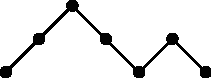
\includegraphics[scale=0.6]{./dyck.pdf} $\ \in$ dyck\_paths(3)
    \end{center} \pause

    \item \tcb{Motzkin Paths}. Same, but you can go horizontally
    \begin{center}
      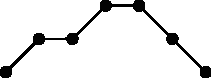
\includegraphics[scale=0.6]{./motzkin.pdf} $\ \in$ motzkin\_paths(6) 
    \end{center}

  \end{itemize}
\end{frame}

\section{Mini tutorial}

\begin{frame}\frametitle{How to install?}
 \begin{itemize}
  \item \textbf{Header-only library}, so no need to install anything (just copy the files to your own project, or anywhere your compiler knows to look for header files).
  \item It does need a somewhat modern C++14 compiler and \href{http://www.boost.org}{\tcb{\underline{boost}}}.
 \end{itemize}
\end{frame}


\subsection{Basic use}

\defverbatim[colored]\combsencillo{\begin{center}
\begin{lstlisting}[language=C++,basicstyle=\ttfamily,keywordstyle=\color{blue},otherkeywords={*,vector,std},commentstyle=\color{MyYellow},tabsize=2]
#include <iostream>
#include "discreture.hpp" //includes everything

using namespace std; 
using namespace dscr;

int main()
{
  for (auto& x : combinations(6,3))
    cout << x << endl;
}
\end{lstlisting}\end{center}
}

\begin{frame}[fragile]\frametitle{Basic use}
To iterate over an object, use standard \texttt{C++} range-based for loop: \pause

 \combsencillo
 
 \pause
 Produces (without the brackets):
  \begin{verbatim} 
  [ 0 1 2 ] [ 0 1 3 ] [ 0 2 3 ]  [ 1 2 3 ] [ 0 1 4 ] 
  [ 0 2 4 ] [ 1 2 4 ] [ 0 3 4 ] [ 1 3 4 ] [ 2 3 4 ] 
  \end{verbatim}

  and just use x[0], x[1], etc. to access the elements.
\end{frame}

\defverbatim[colored]\partsencillo{\begin{center}
\begin{lstlisting}[language=C++,basicstyle=\ttfamily,keywordstyle=\color{blue},otherkeywords={*,vector,std},commentstyle=\color{MyYellow},tabsize=2]
  for (auto& x : partitions(5))
    cout << x << endl; 
\end{lstlisting}\end{center}
}

\begin{frame}[fragile]\frametitle{Another example:}
  \partsencillo
  
  This just prints all ways of adding up to 5 with positive integers:
  \begin{verbatim}
    [ 1 1 1 1 1 ]
    [ 2 1 1 1 ]
    [ 3 1 1 ]
    [ 2 2 1 ]
    [ 4 1 ]
    [ 3 2 ]
    [ 5 ]
  \end{verbatim}
\end{frame}

\defverbatim[colored]\permRA{\begin{center}
\begin{lstlisting}[language=C++,basicstyle=\ttfamily,keywordstyle=\color{blue},otherkeywords={*,vector,std},commentstyle=\color{MyYellow},tabsize=2]
  permutations X(12);
  cout << X[157122128] << endl;
\end{lstlisting}\end{center}
}

\begin{frame}\frametitle{Random Access Iterators}
  Combinations, Permutations and Multisets are ``random access'' containers:
  \permRA
  
  (Instantly) Prints \texttt{[3 11 2 10 9 0 4 1 6 7 5 8]}, which is the 157,122,128-th permutation. \pause
	
	\vspace{0.1cm}
	This allows for pretty easy multi-threaded programs (see included examples).
\end{frame}

\defverbatim[colored]\dyckparen{\begin{center}
\begin{lstlisting}[language=C++,basicstyle=\ttfamily,keywordstyle=\color{blue},otherkeywords={*,vector,std},commentstyle=\color{MyYellow},tabsize=2]
  dyck_paths X(3);
  for (auto& x : X)
    cout << dyck_paths::to_string(x, "()") << endl;  
\end{lstlisting}\end{center}
}

\defverbatim[colored]\motzkinparen{\begin{center}
\begin{lstlisting}[language=C++,basicstyle=\ttfamily,keywordstyle=\color{blue},otherkeywords={*,vector,std},commentstyle=\color{MyYellow},tabsize=2]
motzkin_paths X(6);
for (auto& x : X)
	cout<<motzkin_paths::to_string(x, "(*)")<<endl;  
\end{lstlisting}\end{center}
}

\begin{frame}[fragile]\frametitle{Dyck and Motzkin}
  We can easily generate all correct ways of placing parenthesis:
  \dyckparen
  which prints: \texttt{((()))} $\quad$  \texttt{(()())} $\quad$  \texttt{()(())} $\quad$ \texttt{(())()} $\quad$  \texttt{()()()}
\end{frame}  

% \begin{frame}[fragile]
% O también:
%   \motzkinparen
%   Lo cual imprime:
% \begin{verbatim}    
% ******    ()****    (*)***    *()***    (**)**    
% *(*)**    **()**    (***)*    *(**)*    **(*)*    
% ***()*    (****)    *(***)    **(**)    ***(*)    
% ****()    (())**    (()*)*    ((*))*    (*())*    
% *(())*    (()**)    ((*)*)    (*()*)    *(()*)    
% ((**))    (*(*))    *((*))    (**())    *(*())    
% **(())    ()()**    ()(*)*    ()*()*    (*)()*    
% *()()*    ()(**)    ()*(*)    (*)(*)    *()(*)    
% ()**()    (*)*()    *()*()    (**)()    *(*)()    
% **()()    ((()))    (()())    ()(())    (())()    
%                     ()()()    
% \end{verbatim}
% \end{frame}
    

\subsection{Advanced use}

\defverbatim[colored]\stlsencillo{
\begin{lstlisting}[language=C++,basicstyle=\ttfamily,keywordstyle=\color{blue},otherkeywords={*,vector,std},commentstyle=\color{MyYellow},tabsize=2]
  motzkin_paths X(10);
  std::find_if(X.begin(), X.end(), condition);
\end{lstlisting}
}

\begin{frame}\frametitle{Algorithms}
  We can use standard C++ STL algorithms:
  \stlsencillo
  finds the first motzkin path that satisfies a certain condition.
\end{frame}

\defverbatim[colored]\busqueda{\begin{center}
\begin{lstlisting}[language=C++,basicstyle=\ttfamily,keywordstyle=\color{blue},otherkeywords={*,vector,std},commentstyle=\color{MyYellow},tabsize=2]
// This has almost 10^13 combinations (!)
combinations X(46,23); 

auto it = std::partition_point(X.begin(), X.end(), 
	[](const auto& x) {	
		return x.back() < 36; 
	});
cout << *it << endl;
\end{lstlisting}\end{center}
}

\begin{frame}\frametitle{Standard algorithms}
  You can even do binary search:
  \busqueda
\end{frame}

\defverbatim[colored]\findall{\begin{center}
\begin{lstlisting}[language=C++,basicstyle=\ttfamily,keywordstyle=\color{blue},otherkeywords={*,vector,std},commentstyle=\color{MyYellow},tabsize=2]
  bool no_consecutive(const combination& x)
  {
    int k = x.size();
    return k <= 1 || x[k-2]+1 != x[k-1];
  }
  
  // ...
  
    combinations X(10,5);
    for ( auto& x : X.find_all(no_consecutive) )
      cout << x << endl;
\end{lstlisting}\end{center}
}

\begin{frame}\frametitle{find\_all}
Combinations can even do branch-and-cut: \pause
  \findall
  
  Prints \texttt{[ 0 2 4 6 8 ] [ 0 2 4 6 9 ] [ 0 2 4 7 9 ] ...}, which are combinations that don't have two consecutive numbers.
\end{frame}

\section{Speed}

\begin{frame}\frametitle{Benchmarks}
 \href{https://raw.githubusercontent.com/mraggi/discreture/master/benchmarks.png}{\beamergotobutton{Go to Benchmarks}}

\end{frame}

\defverbatim[colored]\codegsl{\begin{center}
\begin{lstlisting}[language=C++,basicstyle=\ttfamily,keywordstyle=\color{blue},otherkeywords={*,vector,std},commentstyle=\color{MyYellow},tabsize=2]
gsl_combination* c = gsl_combination_calloc(6, 3);
do
{
	// gsl_combination_get(c,i) to obtain the 
	// i-th index
} while (gsl_combination_next(c) == GSL_SUCCESS);
gsl_combination_free(c);
    
\end{lstlisting}\end{center}
}


\begin{frame}\frametitle{How does it compare?} \pause
To generate all combinations in GSL (GNU scientific library), you do:
  \codegsl
  
\end{frame}

\defverbatim[colored]\combsencillodos{\begin{center}
\begin{lstlisting}[language=C++,basicstyle=\ttfamily,keywordstyle=\color{blue},otherkeywords={*,vector,std},commentstyle=\color{MyYellow},tabsize=2]
	for (auto& x : combinations(6,3))
	{
		// x[i] to access
		// i-th index
	}
\end{lstlisting}\end{center}
}

\begin{frame}\frametitle{Easier!}
  \combsencillodos
  
\end{frame}


\begin{frame}\frametitle{What about speed?}\pause
Time to iterate over all $\binom{n}{\left\lfloor n/2 \right\rfloor}$ \pause
  \begin{center}
    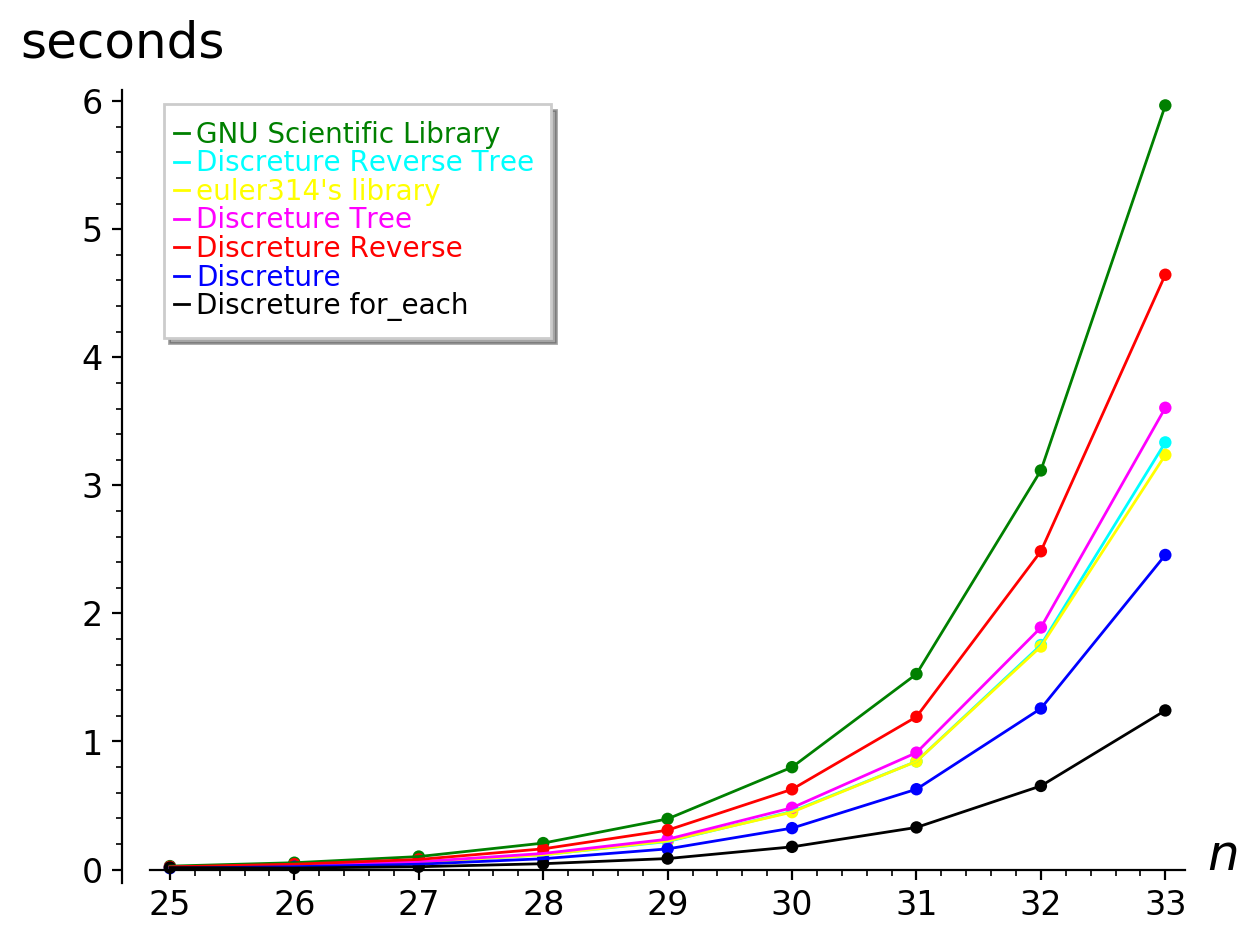
\includegraphics[scale=0.5]{./combvsgsl.png}
  \end{center}
\end{frame}




\begin{frame}\frametitle{Comparisons with sage/gap?}
  \begin{itemize}
    \item \texttt{Sage} and \texttt{GAP} also have many of the combinatorial objects mentioned. \pause
    \item It wouldn't be fair to compare them to discreture (C++ vs python). \pause
    \item For example, in my computer, to see all $\binom{26}{13}$ combinations, \pause
    \begin{itemize}
		\item \texttt{Sage} takes $\approx$34s. \pause
		\item \texttt{GAP} crashes after a while for lack of memory :( \pause Increasing memory limit makes it take $\approx$33s. \pause
    \end{itemize}
    \item Discreture takes $\approx$ 0s.
  \end{itemize}
\end{frame}

\section{Future work}

\begin{frame}\frametitle{Contributing}
\begin{center}
	\begin{tabular}{|c|c|c|c|}
	\hline
	 \textbf{Container} & \textbf{Forward} & \textbf{Reverse} & \textbf{Random Access} \\
	\hline
		Combinations	&  \tcg{Yes}  & \tcg{Yes} & \tcg{Yes}  \\
        Permutations	&  \tcg{Yes}  & \tcg{Yes} & \tcg{Yes}  \\
        Multisets		&  \tcg{Yes}  & \tcg{Yes} & \tcg{Yes}  \\
        Dyck Paths		&  \tcg{Yes}  & \tcr{No } & \tcr{No }  \\
        Motzkin Paths	&  \tcg{Yes}  & \tcr{No } & \tcr{No }  \\ 
        Partitions		&  \tcg{Yes}  & \tcg{Yes} & \tcr{No }  \\ 
        Set Partitions	&  \tcg{Yes}  & \tcr{No } & \tcr{No }  \\
        Compositions    &  \tcr{No }  & \tcr{No } & \tcr{No }  \\
        Graphs (nauty?) &  \tcr{No }  & \tcr{No } & \tcr{No }  \\
        Others? &  \tcr{No }  & \tcr{No } & \tcr{No }  \\
	\hline
	\end{tabular}
\end{center}

\end{frame}

\begin{frame}\frametitle{}
 IF there is time, let's see the solution to Jose Hernández's Problem.
 
 \href{file:/home/mraggi/Dropbox/sources/Mathematics/TestBedForDiscreture/main.cpp}{\beamergotobutton{Go to Jose's Problem}}
 
\end{frame}

\begin{frame}\frametitle{}
\begin{center}
	\huge{Thank you!}
\end{center}
	
	
\huge{\url{github.com/mraggi/discreture}}
\end{frame}




\end{document}

